%%%%%%%%%%%%%%%%%%%%%%%%%%%%%%%%%%%%

\section{対データ}

%%%%%%%%%%%%%%%%%%%%%%%%%%%%%%%%%%%

\subsection{対になった観測値}

\begin{frame}

\dq{「高校とその先」調査から200人の観測値が無作為に抽出された。同じ生徒が読解テストと作文テストを受け、そのスコアを以下に示す。一見して、読解と作文のテストスコアの平均に差があるように見えるか？}

\begin{center}
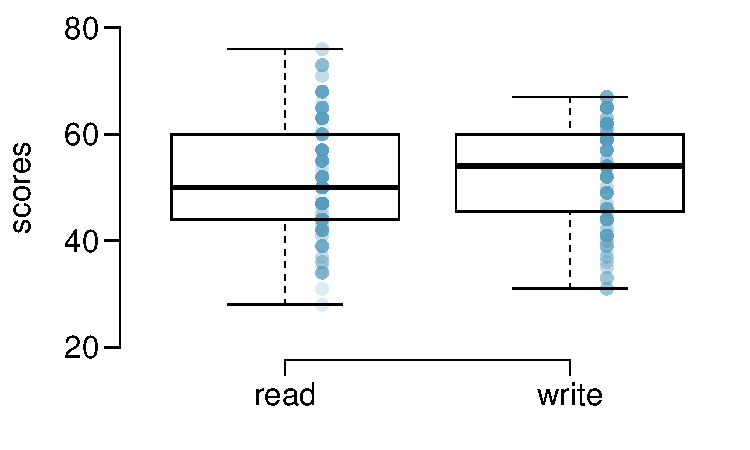
\includegraphics[width=0.5\textwidth]{7-2_paired/figures/hsb2/hsb2_read_write_box}
\end{center}

\end{frame}

%%%%%%%%%%%%%%%%%%%%%%%%%%%%%%%%%%%%

\begin{frame}

\pq{同じ生徒が読解テストと作文テストを受け、そのスコアを以下に示す。各生徒の読解スコアと作文スコアは互いに独立か？}

{\small
\begin{center}
\begin{tabular}{rrrr}
  \hline
 & id & 読解 & 作文 \\
  \hline
1 & 70 & 57 & 52 \\
  2 & 86 & 44 & 33 \\
  3 & 141 & 63 & 44 \\
  4 & 172 & 47 & 52 \\
  $\vdots$ &   $\vdots$  &   $\vdots$ &   $\vdots$  \\
  200 & 137 & 63 & 65 \\
   \hline
\end{tabular}
\end{center}
}

\begin{multicols}{2}
\begin{enumerate}[(a)]
\item はい
\solnMult{いいえ}
\end{enumerate}
\end{multicols}

\end{frame}

%%%%%%%%%%%%%%%%%%%%%%%%%%%%%%%%%%%%

\begin{frame}
\frametitle{対データの分析}

\begin{itemize}

\item 2組の観測値がこのような特別な対応関係（独立でない）を持つとき、それらは\hl{対データ}と呼ばれる。

\item 対データを分析するには、各ペアの観測値の結果の差を見ることが有用である。
\[ \text{差} = \text{読解} - \text{作文} \]

\item 常に一貫した順序で引き算することが重要である。

\end{itemize}

\twocol{0.5}{0.5}{
{\small
\begin{center}
\begin{tabular}{rrrr >{\columncolor[gray]{.9}}r}
  \hline
 & id & 読解 & 作文 & 差 \\
  \hline
1 & 70 & 57 & 52 & 5 \\
  2 & 86 & 44 & 33 & 11 \\
  3 & 141 & 63 & 44 & 19 \\
  4 & 172 & 47 & 52 & -5 \\
  $\vdots$ &   $\vdots$  &   $\vdots$ &   $\vdots$ &   $\vdots$ \\
  200 & 137 & 63 & 65 & -2 \\
   \hline
\end{tabular}
\end{center}
}
}
{
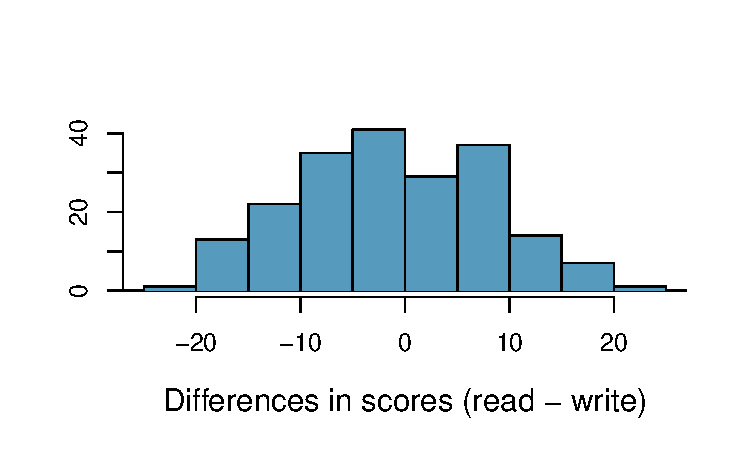
\includegraphics[width=\textwidth]{7-2_paired/figures/hsb2/hsb2_diff_hist}
}

\end{frame}

%%%%%%%%%%%%%%%%%%%%%%%%%%%%%%%%%%%%

\begin{frame}
\frametitle{母数と点推定量}

\begin{itemize}

\item \hl{関心のある母数：}\orange{すべての}高校生の読解スコアと作文スコアの平均差。
\[ \mu_{diff} \]

$\:$ \\

\item \hl{点推定量：}\orange{標本として抽出された}高校生の読解スコアと作文スコアの平均差。
\[ \bar{x}_{diff} \]

\end{itemize}

\end{frame}

%%%%%%%%%%%%%%%%%%%%%%%%%%%%%%%%%%%%

\subsection{対データの推測}

\begin{frame}
\frametitle{仮説の設定}

\dq{読解と作文の試験のスコアに実際に差がないとすれば、平均差はどれくらいと期待されるか？}

\soln{0}

$\:$ \\

\dq{読解と作文の平均スコアに差があるかどうかを検定するための仮説は何か？}

\begin{itemize}
\item[$H_0$:] 読解と作文の平均スコアに差はない。
\[ \mu_{diff} = 0 \]
\item[$H_A$:] 読解と作文の平均スコアに差がある。
\[ \mu_{diff} \ne 0 \]
\end{itemize}

\end{frame}

%%%%%%%%%%%%%%%%%%%%%%%%%%%%%%%%%%%%

\begin{frame}
\frametitle{新しいことは何もない}

\begin{itemize}

\item 分析はこれまでと何ら変わりない。

\item \orange{1つの}標本のデータ（差）を持っている。

\item 平均差が0と異なるかどうかを検定する。

\end{itemize}

\end{frame}

%%%%%%%%%%%%%%%%%%%%%%%%%%%%%%%%%%%%

\begin{frame}
\frametitle{仮定と条件の確認}

\pq{正しいのはどれか？}

\begin{enumerate}[(a)]
\solnMult{生徒は無作為に抽出され、全高校生の10\%未満であるため、標本中のある生徒の読解スコアと作文スコアの差は別の生徒の差と独立であると仮定できる。}
\item 差の分布が二峰性であるため、仮説検定を続けることができない。
\item 差をランダムにするには復元抽出で標本を取るべきであった。
\item 生徒は無作為に抽出され、全生徒の10\%未満であるため、平均差の標本分布はほぼ正規分布になると仮定できる。
\end{enumerate}

\end{frame}

%%%%%%%%%%%%%%%%%%%%%%%%%%%%%%%%%%%

\begin{frame}[shrink]
\frametitle{検定統計量とp値の計算}

\dq{2つのテストの観測された平均スコア差は$-0.545$点、差の標準偏差は$8.887$点であった。$\alpha = 0.05$として、このデータは2つの試験の平均スコアに差があることの説得力ある証拠を提供しているか？}

\twocol{0.5}{0.5}
{
\begin{center}
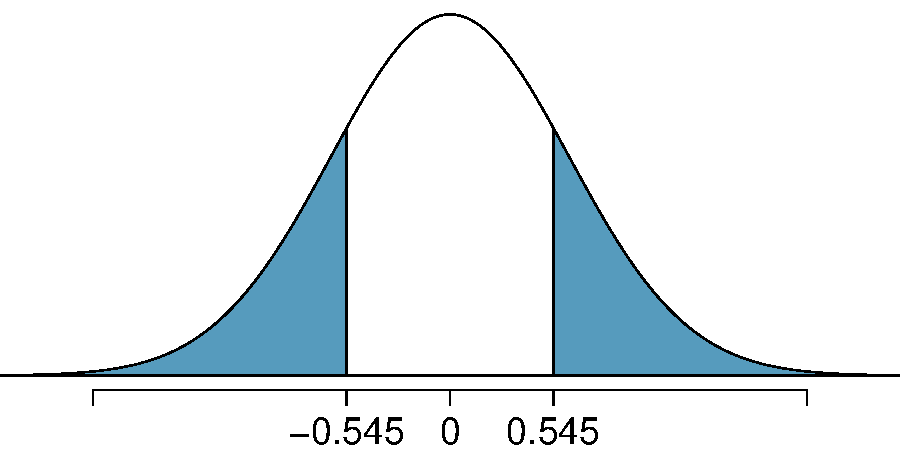
\includegraphics[width=\textwidth]{7-2_paired/figures/hsb2/hsb2_read_write_pval}
\end{center}
}
{
\begin{eqnarray*}
T &=& \frac{-0.545 - 0}{\frac{8.887}{\sqrt{200}}} \\
&=& \frac{-0.545}{0.628} = -0.87 \\
df &=& 200 - 1 = 199 \\
p\text{値} &=& 0.1927 \times 2 = 0.3854
\end{eqnarray*}
}

$\:$ \\
p値$>$0.05であるため、帰無仮説を棄却できない。データは読解と作文の平均スコアに差があることの説得力ある証拠を\underline{提供していない}。

\end{frame}

%%%%%%%%%%%%%%%%%%%%%%%%%%%%%%%%%%%

\begin{frame}
\frametitle{p値の解釈}

\pq{p値の正しい解釈はどれか？}

\begin{enumerate}[(a)]
\item 読解と作文の平均スコアが等しい確率。
\item 読解と作文の平均スコアが異なる確率。
\solnMult{真の平均差が0であると仮定したとき、200人の学生の無作為標本において読解と作文スコアの平均差が（いずれかの方向に）少なくとも0.545となる確率。}
\item 帰無仮説が真であるときに誤って帰無仮説を棄却する確率。
\end{enumerate}

\end{frame}

%%%%%%%%%%%%%%%%%%%%%%%%%%%%%%%%%%%%

\begin{frame}
\frametitle{仮説検定 $\leftrightarrow$ 信頼区間}

\pq{読解と作文スコアの平均差に対する95\%信頼区間を構築するとした場合、この区間は0を含むと期待されるか？}

\begin{enumerate}[(a)]
\solnMult{はい}
\item いいえ
\item 与えられた情報からは判断できない
\end{enumerate}

\soln{
\begin{eqnarray*}
-0.545 \pm 1.97 \frac{8.887}{\sqrt{200}} &=& -0.545 \pm 1.97 \times 0.628 \\
&=& -0.545 \pm 1.24 \\
&=& (-1.785, 0.695)
\end{eqnarray*}
}

\end{frame}

%%%%%%%%%%%%%%%%%%%%%%%%%%%%%%%%%%%%
